\chapter{章节名称}
\section{一级段落名称}
\subsection{二级段落名称}
\subsubsection{三级段落名称}
引用如\upcite{PhysRev.47.777},引用表如表\ref{tab:input_output_r},引用图如图\ref{fig:sample}.

\begin{table}[h]
\small %内容,(五号,宋体/Time new roman)
\centering
\caption{不同频率下的输入和输出阻抗}
\label{tab:input_output_r}
\begin{tabular}{cccc} %表格使用三线表
\toprule %不确定说明中三条线的粗细,待改
频率(Hz) & 1 & 10k & 1M \\
\midrule
输入电阻($\Omega/^\circ$) & 339.719k/-87.84 & 5.6707k/-9.827 & 351.188/-72.377\\
输出电阻($\Omega/^\circ$) & 338.638k/-89.663 & 1.9866k/-1.1228 & 1.9189k/-14.801 \\
\bottomrule
\end{tabular}
\end{table}

\begin{figure}[h]
\centering
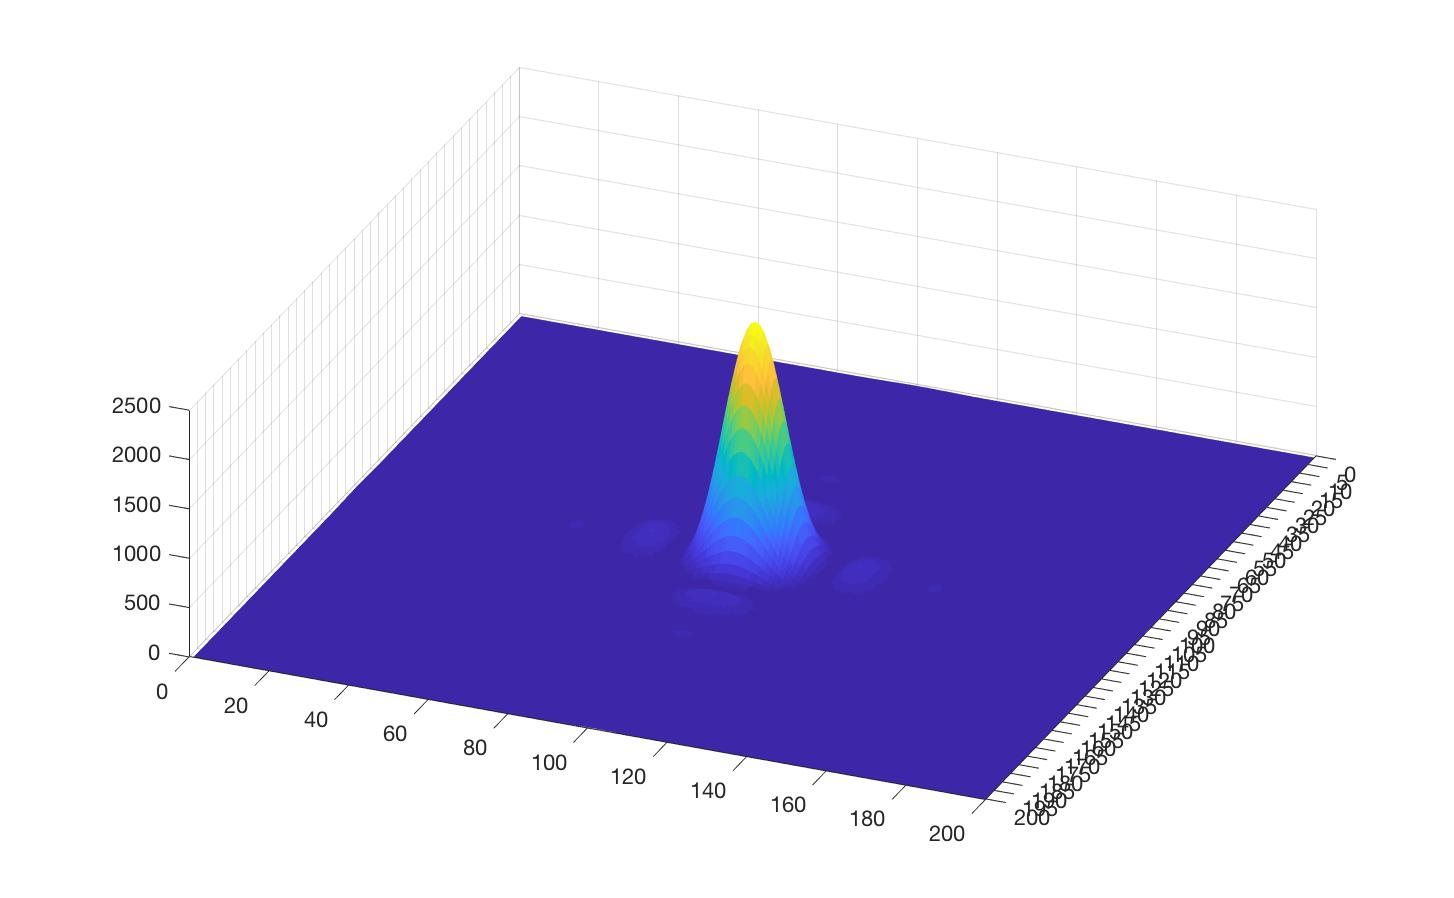
\includegraphics[width=12cm]{Images/Sample.jpg}
\caption{示例图片}
\label{fig:sample}
\end{figure}
\clearpage